\documentclass[10pt,a4paper]{article}

\usepackage[margin=1in]{geometry}
\usepackage[UKenglish]{babel}
\usepackage{enumitem}
\usepackage{calc}
\usepackage{fancyhdr}
\usepackage{graphicx}
\usepackage{multirow}
\usepackage[table]{xcolor}
\usepackage{float}
\usepackage{longtable}
\usepackage{tabularx}
\usepackage{parskip}
\usepackage{soul}
\usepackage{ifthen}
\usepackage[compact]{titlesec}
\usepackage[justification=centering]{caption}
\usepackage{subcaption}
\usepackage{listings}
\usepackage{xcolor}
\usepackage{hyperref}

\colorlet{punct}{red!60!black}
\definecolor{background}{HTML}{EEEEEE}
\definecolor{delim}{RGB}{20,105,176}
\definecolor{key}{RGB}{73,109,112}
\colorlet{numb}{magenta!60!black}

\lstdefinelanguage{json}{
    basicstyle=\normalfont\ttfamily,
    numbers=left,
    numberstyle=\scriptsize,
    stepnumber=1,
    numbersep=8pt,
    showstringspaces=false,
    breaklines=true,
    frame=lines,
    backgroundcolor=\color{background},
    literate=
     *{0}{{{\color{numb}0}}}{1}
      {1}{{{\color{numb}1}}}{1}
      {2}{{{\color{numb}2}}}{1}
      {3}{{{\color{numb}3}}}{1}
      {4}{{{\color{numb}4}}}{1}
      {5}{{{\color{numb}5}}}{1}
      {6}{{{\color{numb}6}}}{1}
      {7}{{{\color{numb}7}}}{1}
      {8}{{{\color{numb}8}}}{1}
      {9}{{{\color{numb}9}}}{1}
      {:}{{{\color{punct}{:}}}}{1}
      {,}{{{\color{punct}{,}}}}{1}
      {\{}{{{\color{delim}{\{}}}}{1}
      {\}}{{{\color{delim}{\}}}}}{1}
      {[}{{{\color{delim}{[}}}}{1}
      {]}{{{\color{delim}{]}}}}{1},
}
\lstset{emph={%  
    Systems, SystemID, Sensors, SensorID, Params, Engines, DatastoreGateway, Reporting
    },emphstyle={\color{key}\bfseries}%
}

\definecolor{reqColor}{RGB}{80,80,120}

%%Tables
\newcommand{\tableformat}[4]{
\begin{table}[ht!]
\centering
  \rowcolors{2}{gray!10} {white}
\def\arraystretch{1.5}
\begin{tabular}{#1}
  \hline
  \rowcolor[gray]{0.9} #2
  \hline
\end{tabular}
\caption{#3}
\label{#4}
\end{table}}

\newcommand{\xtableformat}[4]{
\begin{table}[ht!]
\centering
  \rowcolors{2}{gray!10} {white}
\begin{tabularx}{\textwidth}{#1}
  \hline
  \rowcolor[gray]{0.9} #2
  \hline
\end{tabularx}
\caption{#3}
\label{#4}
\end{table}}

\pagestyle{fancy}
\lhead{T Davies, A Fahie, A Fairbairn, A Free, J Mansfield, R Tucker, M 
Walker}
\chead{}
\rhead{GPIG-C}
\cfoot{\vspace{-0.6cm} \thepage}

\setlist{nolistsep} % Reduces lots of white space around lists

\renewcommand{\headrulewidth}{0.4pt} % Add rules below header
\renewcommand*{\thefootnote}{\fnsymbol{footnote}}

\newcommand{\conreq}[1]{\textcolor{reqColor}{\textbf{CR.#1}}}
\newcommand{\fr}[1]{\textcolor{reqColor}{\textbf{FR.#1}}}
\newcommand{\ed}[1]{\textcolor{reqColor}{\textbf{ED.#1}}}
\newcommand{\nfr}[1]{\textcolor{reqColor}{\textbf{NFR.#1}}}
\newcommand{\qas}[1]{\textcolor{reqColor}{\textbf{QAS.#1}}}

%%Scenarios
\newenvironment{scenario}[1]{
\newcommand{\source}[1]{\item[Source of Stimulus:] ##1}
\newcommand{\stimulus}[1]{\item[Stimulus:] ##1}
\newcommand{\artifact}[1]{\item[Artifact:] ##1}
\newcommand{\environment}[1]{\item[Environment:] ##1}
\newcommand{\response}[1]{\item[Response:] ##1}
\newcommand{\measure}[1]{\item[Response Measure:] ##1}
\newcommand{\rationale}[1]{\item[Scenario Rationale:] ##1}
\newcommand{\quality}[1]{\item[Quality:] ##1}
		\begin{description} [noitemsep]	
		\item[Scenario ID:] \qas{#1}
		}{\end{description} \vspace*{0.3cm}
		}

%%Requirements
\newenvironment{requirements}{
\newcommand{\requirement}[4]{\item[##1{##2}] ##3
							\ifx&##4&
							%nothing
							\else
								\begin{description}
									##4
								\end{description}							
							\fi
							}
		\begin{description}[noitemsep, leftmargin=1.3cm]	
		}{\end{description} \vspace*{0.3cm}
		}
		
\begin{document}
\begin{center}
{\vspace*{-0.7cm}
\Huge GPIG-C HUMS User Manual}
\vspace*{0.3cm}

\end{center}
\vspace*{0.4cm}
\hrule
\vspace*{0.4cm}

\tableofcontents

%-------------------------------------------------------------%
%----------------------LAUNCHING -------------------%
%-------------------------------------------------------------%
\section{Introduction}

The GPIG-C Health and Usage Monitoring System (HUMS) allows systems to be monitored by sensors, which feed information into the core of the HUMS, where it can be stored and analysed, potentially triggering notifications to users if the analysis processes determine that an event of note has occurred. Reports on the state of the system being monitored can be requested by consumers through a web-based administration centre, allowing for a simple interface to the HUMS. This manual will describe how to get a HUMS up and running so that you can start monitoring your own system.

\subsection{Requirements}

To utilise the HUMS, the target system must have Java $7$ installed. This can be obtained for Windows, Linux, and OS X from \url{http://www.java.com/en}.

\section{The HUMS Core}
\label{sec:launching}

\subsection{Launching the core}
\subsubsection{Windows}
To launch the core on Windows, navigate to the directory in Windows Explorer where \texttt{Core.jar} file is located. The core can be launched by double clicking on the \texttt{Core.jar} file. This will launch the HUMS.
\subsubsection{Linux}
To launch the core on linux, using the terminal, navigate to the directory where \texttt{Core.jar} is located. The HUMS can then be launched with the command:
\begin{center}
\texttt{java -jar ./Core.jar}
\end{center}
Alternatively, it can be opened by navigating to the directory containing Core.jar in a file browser. Right click on the file browser and select the option ``Run with Java'' or ``Run with OpenJDK Runtime''.

\subsubsection{OS X}
To launch the core on OS X, using the terminal, navigate to the directory where \texttt{Core.jar} is located. The HUMS can then be launched utilising the command:
\begin{center}
\texttt{java -XstartOnFirstThread -jar Core.jar}
\end{center}

\subsection{Using the Core}
\label{sec:core}

\subsubsection{The User Interface}

When the Core has loaded, the GUI will appear. The functionality for the GUI is set out in Figure~\ref{fig:manualgui}.
\begin{figure}[H]
  \centering
  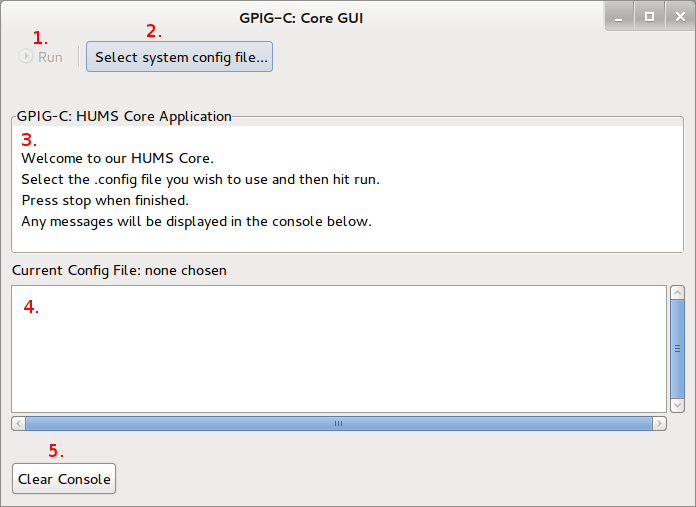
\includegraphics[width=\textwidth]{images/manual-gui.png}
  \caption{The HUMS user interface.}
  \label{fig:manualgui}
\end{figure}
  \begin{enumerate}
\item \textbf{Run Button} \\ 
When a configuration file is loaded, this button runs the core.
\item \textbf{Configuration file select} \\ 
Opens a dialogue box to select the configuration file to be used.
\item \textbf{Core Application Output} \\ 
Displays information from the Core Application itself.
\item \textbf{Current Configuration Output} \\ 
Displays information about things in the configuration file which are being monitored. For example updates and displays when new data is pushed.
\item \textbf{Clear Console Button} \\ 
Clears the \emph{current configuration output}.
\end{enumerate}

\subsubsection{Running with a Given Configuration File}
\label{subsec:loadconf}

To load a configuration file, click the \emph{current configuration output} button ($2$). This will open a dialogue to select the configuration file, navigate to the file, select it and click ``Open''. The \emph{Run Button} should now be clickable. Once clicked the GUI will load the configuration file, initialise the core with the appropriate engines and the \emph{Run Button} will become a \emph{Stop Button}.

\subsubsection{Loading a Different Configuration at Runtime}

Click the \emph{Stop Button}, which is located at the same position as the \emph{Run Button} ($1$). This will halt the running of the core for the current configuration, and will revert the GUI back to the same state as when it was first launched. The steps for Section~\ref{subsec:loadconf} can then be repeated for a different, or updated, configuration file.

\section{Demonstration}
\label{subsec:demo}
\subsection{Launching the Demonstration for the Emitters}
\subsubsection{Windows}
To launch the emitter demo on Windows, navigate to the directory in Windows Explorer where \texttt{EmitterLauncher.jar} file is located. The emitter demo can be launched by double clicking on the \texttt{EmitterLauncher.jar} file. This will launch the emitter demo.
\subsubsection{Linux}
To launch the emitter demo on linux, using the terminal, navigate to the directory where \texttt{EmitterLauncher.jar} is located. The emitter demo can then be launched with the command:
\begin{center}
\texttt{java -jar ./EmitterLauncher.jar}
\end{center}
Alternatively, it can be opened by navigating to the directory containing EmitterLauncher.jar in a file browser. Right click on the file browser and select the option ``Run with Java'' or ``Run with OpenJDK Runtime''.

\subsubsection{OS X}
To launch the emitter demo on OS X, using the terminal, navigate to the directory where \texttt{EmitterLauncher.jar} is located. The emitter demo can then be launched utilising the command:
\begin{center}
\texttt{java -XstartOnFirstThread -jar EmitterLauncher.jar}
\end{center}

\subsection{Demo GUI}
\begin{figure}[H]
  \centering
  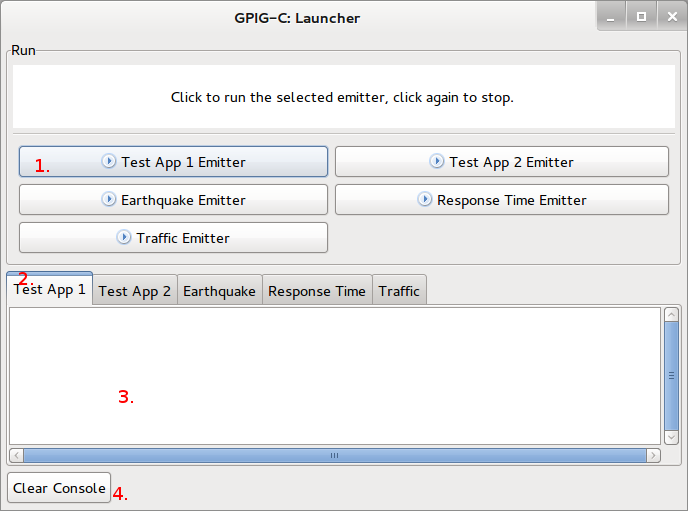
\includegraphics[width=\textwidth]{images/demo-gui.png}
  \caption{The GUI for the Demonstration of the monitoring and analysis systems for our HUMS.}
  \label{fig:demogui}
\end{figure}
\begin{enumerate}
\item \textbf{Application Runners} \\ For each configuration for demonstration there is a button to run it. The output for each different demonstration is shown in the \emph{output area} ($3$).
\item \textbf{Output Selection Tabs} \\ For each configuration file, there is a matching output. These tabs select which output is displayed in the\emph{output area}.
\item \textbf{Output area} \\ Displays the currently selected configuration files output. Updates on events, such as new information being sent into the core.
\item \textbf{Clear Console Button} \\ 
Clears the current configuration's \emph{output area} ($3$).
\end{enumerate}

\section{Troubleshooting}

\subsection{Unsupported major.minor version 51.0}

If there is an error which reads unsupported major.minor version. This means that the version of Java installed on your machine is not up to date. Therefore, to be able to run the HUMS system, you will have to install a newer version of Java. The lowest version of Java which is supported is Java $7$, versions $6$ or lower will give an error of this nature.

\end{document}
